%%
%% This is file `mcmthesis-demo.tex',
%% generated with the docstrip utility.
%%
%% The original source files were:
%%
%% mcmthesis.dtx  (with options: `demo')
%%
%% -----------------------------------
%%
%% This is a generated file.
%%
%% Copyright (C)
%%       2010 -- 2015 by Zhaoli Wang
%%       2014 -- 2019 by Liam Huang
%%       2019 -- present by latexstudio.net
%%
%% This work may be distributed and/or modified under the
%% conditions of the LaTeX Project Public License, either version 1.3
%% of this license or (at your option) any later version.
%% The latest version of this license is in
%%   http://www.latex-project.org/lppl.txt
%% and version 1.3 or later is part of all distributions of LaTeX
%% version 2005/12/01 or later.
%%
%% This work has the LPPL maintenance status `maintained'.
%%
%% The Current Maintainer of this work is Liam Huang.
%%
%%
%% This is file `mcmthesis-demo.tex',
%% generated with the docstrip utility.
%%
%% The original source files were:
%%
%% mcmthesis.dtx  (with options: `demo')
%%
%% -----------------------------------
%%
%% This is a generated file.
%%
%% Copyright (C)
%%       2010 -- 2015 by Zhaoli Wang
%%       2014 -- 2019 by Liam Huang
%%       2019 -- present by latexstudio.net
%%
%% This work may be distributed and/or modified under the
%% conditions of the LaTeX Project Public License, either version 1.3
%% of this license or (at your option) any later version.
%% The latest version of this license is in
%%   http://www.latex-project.org/lppl.txt
%% and version 1.3 or later is part of all distributions of LaTeX
%% version 2005/12/01 or later.
%%
%% This work has the LPPL maintenance status `maintained'.
%%
%% The Current Maintainer of this work is Liam Huang.
%%
\documentclass{mcmthesis}
\mcmsetup{CTeX = false,    % 使用 CTeX 套装时，设置为 true
          tcn = {5049}, problem = \textcolor{red}{B},
          sheet = true, titleinsheet = true, keywordsinsheet = true,
          titlepage = false, abstract = false}
\usepackage{newtxtext}     % \usepackage{palatino}
\usepackage[numbers]{natbib}
\usepackage{tocloft}
\usepackage{tabularx}
\usepackage{makecell}
\usepackage{float}
\usepackage{subcaption}
\usepackage{graphicx}
\usepackage{gensymb}
\usepackage{xcolor}
\usepackage{soul}
\usepackage{hyperref}
\usepackage{etoolbox}
\hypersetup{
  colorlinks=true,
  linkcolor=blue,   % 正文交叉引用（\ref, \autoref）为蓝色
  citecolor=red,
  urlcolor=black
}




% Force English abstract heading even when ctex is loaded.
%\ctexset{abstractname = {Summary}}
\renewcommand{\abstractname}{Summary}

\sethlcolor{yellow!40}
\newcommand{\hltext}[1]{\colorbox{yellow!40}{#1}}
\setlength{\cftbeforesecskip}{6pt}
\renewcommand{\contentsname}{\hspace*{\fill}\Large\bfseries Contents \hspace*{\fill}}

\title{Deep-Sea Exploration: Positioning, Search, and Rescue of Manned Submersibles}
% \author{\small \href{http://www.latexstudio.net/}
%   {
\includegraphics[width=7cm]{mcmthesis-logo}}}
\date{\today}

\begin{document}

\begin{abstract}
The Greek company MCMS aims to deploy its manufactured submersibles for manned deep-sea exploration missions.
To ensure the safety of the personnel involved in this project, this paper develops \textbf{a position prediction and search planning framework}
based on the dynamic characteristics of submersibles operating in deep-sea environments
under different failure scenarios,
providing actionable guidance for rescue operations and promoting the sustainable development of deep-sea exploration projects.

\textbf{For Problem 1}, we collected data on Ionian Sea seawater depth and ocean currents to construct a \textbf{drift dynamics model} that includes gravity, buoyancy, and hydrodynamic resistance.
Subsequently, we used \textbf{Monte Carlo simulations} to quantify the impact of current prediction errors, turbulence, and model uncertainties on position dispersion. 
The results show that under neutral buoyancy conditions, \textbf{the positioning uncertainty is highly sensitive to the deviation in current prediction}. 
By equipping the submersible with a \textbf{USBL} (Ultra Short Baseline) system and an \textbf{IMU} (Inertial Measurement Unit) to transmit position and speed data to the support vessel, and using an \textbf{ADCP} (Acoustic Doppler Current Profiler) system to measure surrounding ocean currents, this uncertainty can be effectively reduced.

\textbf{For Problem 2}, \textbf{a multi-objective optimization model} balancing performance, cost, and engineering constraints was established to minimize deployment cost while maximizing 
detection probability. We found that a configuration consisting of \textbf{a towed sonar and a high-end AUV} (Autonomous Underwater Vehicle) achieves 
\textbf{a $99.87\%$ rescue success rate within a $90{,}000$ budget}, while additional sonar systems further enhance reliability in high-risk missions.

\textbf{For Problem 3}, we introduced \textbf{Bayesian search theory}, incorporating the observations of the support vessel and sensor scanning results into consideration,
to continuously update the posterior probability distribution of the underwater vehicle's position.
Then, based on the criterion of maximizing the probability of detecting the underwater vehicle per unit time, \textbf{an adaptive heading decision-making strategy} was implemented.
Under conditions of limited time and budget, this method significantly improved the detection efficiency,
\textbf{achieving a rescue success rate of 70\% within 10 hours and 90\% within 30 hours.}

\textbf{For Problem 4}, the search task was expanded from \textbf{a single-target scenario to a multi-target scenario}.
 We proposed \textbf{a hierarchical search mechanism}.
At the upper level, path optimization based on the high-probability target center was used to reduce the target switching time;
At the lower level, a spiral coverage mode matching the sensor scanning width was adopted to systematically clear the confidence region.
This method avoided \textbf{oscillations and local optima caused by greedy strategies},
and dynamically reduced the search space through Bayesian updates.
The results showed that when searching for three underwater targets,
\textbf{the success probability could be increased to 87\% within 11 hours}.
Furthermore, the proposed mechanism showed a gradually increasing trend in success probability in multi-target scenarios,
indicating its \textbf{strong scalability}.


\begin{keywords}
Monte Carlo \quad Bayesian search \quad manned submersible \quad deep-sea exploration \quad localization and search
\end{keywords}
\end{abstract}

\maketitle

%% Generate the Table of Contents, if it's needed.
% \renewcommand{\contentsname}{\centering Contents}.
\pretocmd{\tableofcontents}{%
  \hypersetup{linkcolor=black}%
}{}{}
\apptocmd{\tableofcontents}{%
  \hypersetup{linkcolor=blue}%
}{}{}
\thispagestyle{fancy}
\tableofcontents        % 若不想要目录, 注释掉该句



\newpage









\section{Introduction}
\subsection{Restatement of the Problem}
Nowadays, people are keen on embarking on deep-sea exploration journeys to satisfy their endless curiosity and pursue adventurous experiences.
Therefore, MCMS hopes that the submersibles they manufacture can help people explore the seabed of the Ionian Sea and find shipwrecks.
\begin{figure}[H]
  \centering  
  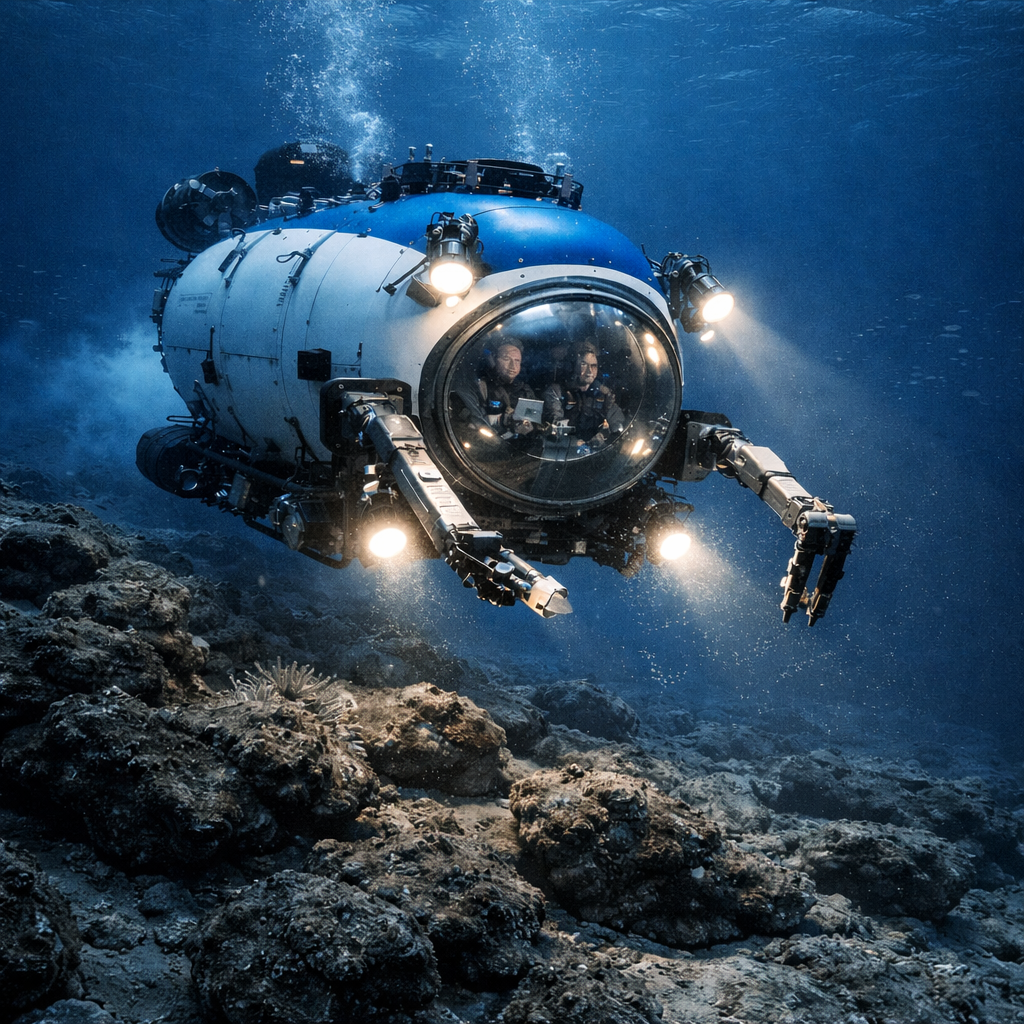
\includegraphics[width=0.4\textwidth]{figures/background.png}
  \caption{Deep-sea Submersible}
\end{figure}
\vspace{-0.4cm}

After being transported to the designated location by the mother ship, the submersible will operate independently in the deep sea.
However, influenced by ocean currents, varying densities in the ocean, and seabed topography, it may encounter a series of challenges during deep-sea exploration, including communication interruptions and propulsion system failures.
Therefore, ensuring the safety of the submersible during its journey, equipping the mother ship with appropriate search equipment and algorithms;
equipping the submersible with communication devices and establishing location prediction models are key to solving this problem.
Based on the above understanding, this study will attempt to address the following issues:
\begin{itemize}
  \item \textbf{Problem 1} Establish a model to predict the changing position of the submersible over time, while assessing the uncertainty of this prediction,
        and determine what information the submersible needs to send periodically to reduce this uncertainty.
  \item \textbf{Problem 2} Considering the availability, maintenance, preparation, and usage costs of additional search equipment, recommend suitable additional search equipment.
  \item \textbf{Problem 3} Using the established location information model, recommend initial deployment points and search patterns for the equipment to minimize the time the submersible is lost, while
       establishing a probability function for the submersible being found as time elapses and search results accumulate.
  \item \textbf{Problem 4} Extend the model to other tourist destinations, such as the Caribbean Sea.
  Additionally, adjust and modify the model to accommodate multiple submersibles operating within the same general area.
\end{itemize}



\subsection{Literature Review}
Early underwater search models originated from operational research applied during the search for the wreckage of the submarine Scorpion, 
where Richardson first applied probabilistic theory, treating the lost submersible as a probabilistic target with an unknown location, thereby laying the foundation for probability-based underwater search methods \cite{SCORPION}.

This framework was further refined during the search for Air France Flight AF 447. Stone and Colleen M. Lawrence adopted a Bayesian approach to integrate heterogeneous information sources, including the last known position, drift models, and the outcomes of previous unsuccessful searches, in order to iteratively update the posterior probability distribution of the wreckage location \cite{AF447}. By representing potential trajectories with particles and suppressing probabilities in searched areas through Bayesian updating, their work demonstrated that probabilistic motion modeling combined with Bayesian search provides a robust and practical framework for underwater target localization under severe uncertainty.

Effective underwater search also relies critically on appropriate sensing and navigation equipment, as GPS signals cannot propagate underwater \cite{pmid34883851}.
The Inertial Navigation System (INS) serves as a fundamental navigation solution by integrating acceleration and angular rate measurements to estimate position and velocity, though its errors accumulate over time and require periodic correction \cite{app14219671,8943978}. 
To mitigate drift, Doppler Velocity Logs (DVLs) are commonly integrated with INS, significantly improving localization accuracy. In addition, Ultra Short Baseline (USBL) systems enable real-time tracking of underwater vehicles from surface vessels, albeit with accuracy degradation over long distances \cite{rs16010199}. 
Furthermore, Acoustic Doppler Current Profilers (ADCPs) are widely employed to measure depth-dependent ocean currents, providing essential environmental inputs for predicting underwater vehicle drift trajectories.
\subsection{Our Work}
Inspired by the aforementioned research and in order to address the aforementioned issues, our specific workflow is illustrated in \autoref{fig:Workflow}.
\vspace{-0.5cm}
\begin{figure}[H]
    \centering
    
\includegraphics[width=1\textwidth]{figures/our.png}
    \caption{Our Workflow}
    \label{fig:Workflow}
\end{figure}
\section{Assumptions and Justification}
\textbf{Assumption 1:}
The missing submersible is assumed to have reported its status to the mother ship every 15 minutes prior to loss of contact, and signal transmission delay is neglected.

According to relevant design standards \cite{IMO2021Submersible} and 
the 2023 Titan incident investigation \cite{USCG2023Titan}, 
the communication interval is set to 15 minutes. With a maximum separation of 10 km and an acoustic speed of 1500 m/s, 
the transmission delay is about $6.67,\text{s}$. Assuming a drift speed of $1.5,\text{m/s}$ after power loss, the induced position error is approximately 10 m, which is negligible relative to the sonar scanning width.

\textbf{Assumption 2:}
The motion of the submersible is modeled as a three-degree-of-freedom translational system, while its attitude dynamics are neglected.

Only translational motion is considered, since post-failure attitude effects are passively stabilized and negligible relative to ocean currents and buoyancy.

\textbf{Assumption 3:}
After mechanical failure and loss of communication, the submersible is assumed to be either drifting under near-neutral buoyancy or resting on the seabed.

Following power loss, the motion rapidly becomes passive and dominated by buoyancy and environmental forces. The transient phase is short, allowing the long-term behavior to be simplified into two mutually exclusive steady-state scenarios: depth-level drifting or continuous sinking until seabed settlement.

\textbf{Assumption 4:}
Search operations are conducted under favorable weather conditions with the sea state not exceeding Level~3.

Under this condition, the influence of surface wind on the mother ship is negligible, and the effects of surface waves on deep-sea currents and submersible motion are ignored.
To maximize personnel safety,
the deployment of rescue ships and equipment must be carried out under safe sea conditions,
to ensure better operation of the submersible and normal deployment and operation of the search equipment.
\vspace{-0.1cm}
\section{Notations}
\vspace{-0.3cm}
\begin{table}[H]
\centering
\caption{Notations used in this paper}
\vspace{-0.4cm}
\begin{tabularx}{0.8\textwidth}{cXc}
\toprule
Symbol & Description & Unit \\
\midrule
$(x,y,z,t)$ & North-East-Down (NED)  and time & m, m, m, s \\
$\bm{X}=[x,y,z]^T$ & Submersible position vector & m \\
$\dot{\bm{X}}$ & Submersible velocity vector & m/s \\
$g$ & Gravitational acceleration & m/s$^2$ \\
$\rho_s$ & Submersible density & kg/m$^3$ \\
$\rho_o$ & Ocean density & kg/m$^3$ \\
$\bm{F}_G$ & Gravitational force & N \\
$\bm{F}_D(z,\dot{\bm{x}})$ & Drag force & N \\
$\bm{v}_{\mathrm{current}}(z)$ & Ocean current velocity field & m/s \\
$H(x, y)$ & Seafloor topography & m \\
$Sp$ & Search path & - \\
$P_d$ & Probability of device detecting the target & - \\
$P_s(t)$ & Cumulative search success rate & - \\
$T$ & Search time & h \\
\bottomrule
\end{tabularx}
\end{table}
\section{Dynamics Model of the Submersible in the Deep Sea}
In the real ocean environment, the spatial distribution of seafloor topography, straits, and islands significantly affects the flow and exchange processes of the water body.
Variations in ocean depth lead to different regions receiving varying intensities of solar radiation,
resulting in spatial heterogeneity in seawater temperature and salinity.
These factors collectively result in seawater density to vary with depth, temperature, and salinity.

The calculation of seawater density uses the EOS-80 (Equation of State 1980) state equation.
Under standard atmospheric pressure conditions, the density of pure water can be expressed as a fifth-degree polynomial of temperature $T$:
\begin{equation}
\rho_w = a_0 + a_1 T + a_2 T^2 + a_3 T^3 + a_4 T^4 + a_5 T^5 ,
\end{equation}
On this basis, the density of seawater under standard atmospheric pressure can be expressed as a function of salinity $S$ and temperature $T$:
\begin{equation}
\rho(S,T,0)=\rho_w
+ S \left( b_0 + b_1 T + b_2 T^2 + b_3 T^3 + b_4 T^4 \right)
+ S^{3/2} \left( c_0 + c_1 T + c_2 T^2 \right)
+ d_0 S^2 ,
\end{equation}
where $S$ represents the salinity of seawater.

Further considering the pressure effects in the deep-sea environment, a pressure correction term is introduced, and the seawater density can be expressed as:
\begin{equation}
\rho(S,T,p)=\frac{\rho(S,T,0)}{1-\dfrac{p}{K(S,T,p)}} ,
\end{equation}
where $p$ is the hydrostatic pressure, and $K(S,T,p)$ is the bulk modulus (shear modulus), which characterizes seawater's resistance to compression and increases with pressure.
To closely approximate real conditions, this paper selects measured ocean environmental data from the Ionian Sea from August 1 to August 7, 2025, as input conditions to characterize the submersible's motion behavior in the actual deep-sea environment.

Under the premise of a relatively small study area scale and relatively gentle environmental parameter changes, we linearize the seawater equation of state within a local range to obtain an approximate linear relationship of seawater density with salinity $S$, temperature $T$, and depth $z$, to support subsequent calculations of the submersible's dynamics and drift models.
\begin{equation}
  \rho(z)\approx1000+0.8(S-35)-0.2(T-20)+0.004z
\end{equation}

In the deep sea, the submersible's volume is affected by pressure and temperature, and can be expressed as:
\begin{equation}
  V(z)=V_0(1-\alpha\cdot P(z)-\beta\cdot\Delta T(z))
\end{equation}
where $V_0$ is the initial volume. $\alpha\approx9.1\times10^{-11}\,\mathrm{Pa}^{-1}$ is the compressibility coefficient of the titanium alloy material used in the submersible.
$\beta\approx2.6\times10^{-5}\,\mathrm{K}^{-1}$ is the thermal expansion coefficient of the titanium alloy material used in the submersible.
From this, we can obtain the relationship between the submersible's buoyancy and depth as:
\begin{equation}
  \bm{F}_{B}({z})=[0,0,-g\cdot\rho(z)\cdot V(z)]^{\mathrm{T}}
\end{equation}

We use a parameter $M$ to represent the weight of the submersible (including dry weight and ballast water).
Due to the differences in the geometric shapes of the submersible in the horizontal and vertical directions,
the additional mass generated when it interacts with the surrounding fluid also has directionality.
Therefore, this paper adopts an anisotropic mass model, and its equivalent mass matrix is expressed as
\begin{equation}
  M_{sys} = \left[
  \begin{matrix}
    M + m_{a,xy} & 0 & 0 \\
    0 & M + m_{a,xy} & 0 \\
    0 & 0 & M + m_{a,z}
  \end{matrix}
  \right]
\end{equation}
where $m_{a,xy},m_{a,z}$ represent the added mass in the horizontal and vertical directions, respectively, reflecting anisotropy.

The drift of the submersible after losing propulsion is mainly driven by ocean currents.
Similarly, this paper constructs a depth-varying ocean current velocity field $\bm{v}_{current}(z)$ based on actual ocean current data from the Ionian Sea from August 1 to 7, 2025.
Due to the relative motion between the submersible's absolute velocity and the surrounding fluid velocity,
this relative velocity induces fluid drag.
According to the quadratic drag law, the drag force can be expressed as
\begin{equation}
  \begin{matrix}\bm{F}_D&=\frac{1}{2}\rho(z)\mathbf{C}_D\odot\mathbf{A}\odot(|\mathbf{v}_{rel}|\circ\mathbf{v}_{rel})\\\end{matrix}
\end{equation}
where
$\odot$ represents Hadamard product (multiplication of corresponding elements).
$\mathbf{v}_{rel}$ represents the velocity vector of the submersible relative to the ocean current. $\mathbf{v}_{rel}=\bm{v}_{current}(z)-\dot{\bm{X}}$,
$\bm{v}_{current}(z)$ represents the ocean current field related to depth.
$\mathbf{A}$ is the characteristic reference area vector.
$\mathbf{C}_D$ is the drag coefficient vector.

We use $F_G=[0,0,Mg]^T$ to represent the weight of the submersible. Taking the initial position of the submersible as the origin, we establish a North-East-Down (NED) inertial coordinate system,
and define the position vector of the submersible as $\bm{X}=[x,y,z]^T$.
Finally, according to Newton's second law, the equation of motion of the submersible can be expressed as:
\begin{equation}
M_{\mathrm{sys}}\dot{\bm{X}} = \bm{F}_{G} + \bm{F}_{B}(z) + \bm{F}_{D}({z},\dot{\bm{X}}) 
\end{equation}


\section{Solution to Problem 1}
We utilized a real-world Titan submersible model as our reference, taking its shape and weight as the basis for our study, and thereby constructing the dynamics model of the submersible.
The parameters of this submarine are shown in \autoref{tab:sub_parameters}.
\begin{table}[htbp]
\centering
\caption{Main Physical Parameters of the Submersible}
\vspace{-0.4cm} \label{tab:sub_parameters}
\begin{tabularx}{\linewidth}{XXXX}
\toprule
Parameter Name & Symbol & Value & Unit \\
\midrule
Total Mass & $m$ & 10,432 & kg \\
Length  & $L$ & 6.7 & m \\
Width  & $W$ & 2.8 & m \\
Height & $H$ & 2.5 & m \\
Maximum Speed & $v_{\max}$ & 1.5& m/s  \\
Diving Speed & $v_{\text{desc}}$ & 50 & m/min \\
Passenger Capacity & $N_{\text{pax}}$ & 5 & - \\
Life Support & $T_{\text{lim}}$ & 96 & hours  \\
\bottomrule
\end{tabularx}
\end{table}
These parameters are mainly used to estimate the force characteristics of the submersible in the fluid,
the reference area facing the flow, and the system inertia, providing basic input for subsequent dynamics and trajectory prediction models.
According to the problem statement, the final motion states of the submersible after failure mainly include
neutral buoyancy suspension and sinking to the seabed.

When the submersible is ultimately in a state of neutral buoyancy,
its average density is insufficient to continue sinking,
and the submersible will hover at a certain stable depth.
At this time, the buoyancy acting on the submersible in the vertical direction balances its weight,
$F_G=F_B(z)$, while it continues to move horizontally due to the influence of ocean currents.
Another scenario is that the submersible experiences flooding due to mechanical failure during underwater operations,
resulting in a significant increase in its overall density,
causing its weight to exceed buoyancy and continue sinking,
eventually contacting the seabed and causing a grounding accident.
In this case, the submersible no longer undergoes significant displacement after reaching the seabed,
and the grounding position becomes the final resting place of the faulty submersible.
\subsection{Stochastic Lagrangian Particle Tracking Model}
The problem requires predicting the spatial position of the submersible after losing contact from the perspective of safety and search and rescue.
Therefore, the core of this problem is to characterize the stochastic motion trajectory of the submersible without propulsion capability in three-dimensional space.
Based on the aforementioned dynamic model, this paper further introduces probabilistic methods to handle environmental uncertainty and fault randomness.
The outcomes after submersible failure can be categorized into two types:
one is hovering at a certain neutral depth,
and the other is continuous sinking and eventually settling on the seabed.
However, the specific depth and type of failure of the submersible are random in practice,
making it difficult to directly provide deterministic solutions.
Therefore, we introduce probabilistic modeling ideas in the trajectory prediction process,
constructing a stochastic Lagrangian particle tracking model
that combines deterministic ocean flow fields with random disturbances to simulate possible motion paths of the submersible in a complex marine environment.

\textbf{Uncertainty Initialization:}
To characterize the uncertainty of the submersible failure depth,
we use a Gaussian Mixture Model (GMM)
to model the initial depth distribution of the submersible under different failure modes,
distinguishing between the two typical scenarios of neutral hovering and sinking.
Its probability density function is expressed as
\begin{equation}
P(z)
=
w_{\mathrm{hover}}
\cdot
\mathcal{N}\!\left(z \mid \mu_h, \sigma_h^2 \right)
+
w_{\mathrm{sink}}
\cdot
\mathcal{N}\!\left(z \mid \mu_s, \sigma_s^2 \right),
\end{equation}
where
$\mathcal{N}(z \mid \mu, \sigma^2)$ denotes a one-dimensional normal distribution with mean $\mu$ and variance $\sigma^2$,
$w_{\mathrm{hover}}$ and $w_{\mathrm{sink}}$ correspond to the weight coefficients for the submersible's final hovering and sinking states, respectively,
and satisfy
$w_{\mathrm{hover}} + w_{\mathrm{sink}} = 1$.

\vspace{0.5em}
\textbf{Trajectory Integration Model:}
Under the given initial conditions,
the trajectory of the submersible is calculated through discrete-time integration.
Its continuous-time velocity model can be uniformly expressed as
\begin{equation}
\dot{\mathbf{X}}(t)
=
\alpha \cdot \mathbf{V}_{\mathrm{pre}}(\mathbf{X}(t))
+
\mathbf{V}_{\mathrm{sys}}
+
\mathbf{V}_{\mathrm{turb}}(t),
\end{equation}
where
$\mathbf{X}(t) = [x(t),y(t)]^{\mathrm{T}}$ represents the spatial position of the underwater vehicle in the horizontal plane.
$\mathbf{V}_{\mathrm{pre}}$ is the basic predicted ocean current velocity field provided by the numerical ocean model.
$\alpha$ is the speed scaling coefficient.
$\mathbf{V}_{\mathrm{sys}}$ and $\mathbf{V}_{\mathrm{turb}}(t)$ respectively represent the systematic ocean current prediction deviation and the random turbulent disturbance term.

\vspace{0.5em}
\subsection{Monte Carlo Uncertainty Model}
In the actual marine environment,
the uncertainty in predicting the position of the submersible not only arises from the randomness of the failure event itself,
but is also significantly affected by errors in ocean current field predictions.
Since ocean current data is usually based on numerical forecasts and discrete observations,
and spatially filled through methods such as vertical nearest neighbor interpolation,
inevitable model errors and observation noise are introduced.
Therefore,
in multiple failure scenario replays,
the actual ocean current field acting on the submersible should be regarded as a random variable rather than a deterministic input.

Based on the idea of Monte Carlo simulation,
we model the ocean current velocity as the superposition of three components:
\begin{equation}
\mathbf{V}_r(x,y,z,t)
=
\mathbf{V}_{\mathrm{pre}}(x,y,z)
+
\mathbf{V}_{\mathrm{sys}}^{(k)}
+
\mathbf{V}_{\mathrm{turb}}(t),
\end{equation}
where
$\mathbf{V}_{\mathrm{sys}}^{(k)}$ is the systematic error term introduced in the $k$-th Monte Carlo simulation,
used to characterize the bias of ocean current prediction on the overall scale.
This term remains constant within a single simulation,
but follows a zero-mean normal distribution across different simulations:
\begin{equation}
\mathbf{V}_{\mathrm{sys}}
\sim
\mathcal{N}\!\left( \mathbf{0}, \sigma_{\mathrm{sys}}^{2} \right),
\qquad
\sigma_{\mathrm{sys}} \approx 0.1\,\mathrm{m/s}.
\end{equation}

Random turbulent term $\mathbf{V}_{\mathrm{turb}}(t)$
is used to describe time-correlated random disturbances caused by small-scale ocean turbulence,
and is assumed to follow a zero-mean normal distribution:
\begin{equation}
\mathbf{V}_{\mathrm{turb}}(t)
\sim
\mathcal{N}\!\left( \mathbf{0}, \sigma_{\mathrm{turb}}^{2} \right),
\qquad
\sigma_{\mathrm{turb}} \approx 0.02\,\mathrm{m/s}.
\end{equation}

Under the above assumptions,
the discrete-time state update equation of the submersible in the $k$-th Monte Carlo simulation is uniformly expressed as
\begin{equation}
\mathbf{X}_{t+\Delta t}
=
\mathbf{X}_t
+
\left(
\alpha \cdot \mathbf{V}_{\mathrm{pre}}(\mathbf{X}_t)
+
\mathbf{V}_{\mathrm{sys}}^{(k)}
+
\mathbf{V}_{\mathrm{turb}}(t)
\right)\Delta t.
\end{equation}

By performing $N$ repeated simulations of the above state equation,
a sample set of potential submersible landing points can be obtained.
In a statistical sense,
we use a two-dimensional multivariate normal distribution to approximate the distribution of landing points,
with its covariance matrix defined as
\begin{equation}
\Sigma
=
\begin{bmatrix}
\mathrm{Var}(x) & \mathrm{Cov}(x,y) \\
\mathrm{Cov}(y,x) & \mathrm{Var}(y)
\end{bmatrix}.
\end{equation}

To quantify the uncertainty in the submersible's position,
we define the uncertainty region $S_{\mathrm{UQ}}$
as the $95\%$ confidence ellipse under the two-dimensional normal distribution,
whose area can be expressed as
\begin{equation}
S_{\mathrm{UQ}}
=
\pi
\sqrt{ \chi_{0.95,2}^{2} \lambda_1 }
\sqrt{ \chi_{0.95,2}^{2} \lambda_2 },
\end{equation}
where
$\lambda_1,\lambda_2$ are the eigenvalues of the covariance matrix ${\Sigma}$,
and
$\chi_{0.95,2}^{2} \approx 5.991$
is the critical value of the chi-square distribution with 2 degrees of freedom at the 95\% confidence level.
\subsection{Result Analysis}
Based on the above established model,
we plotted the true terrain structure of the Ionian Sea region from both three-dimensional and vertical profile perspectives,
as shown in \autoref{fig:ionian-sea}. At the same time, we calculated the depth of the submarine hover point to be $2000.6m$.
\begin{figure}[htbp]
  \centering
  % ===== 左侧：海底地形 =====
  \begin{subfigure}[b]{0.48\linewidth}
    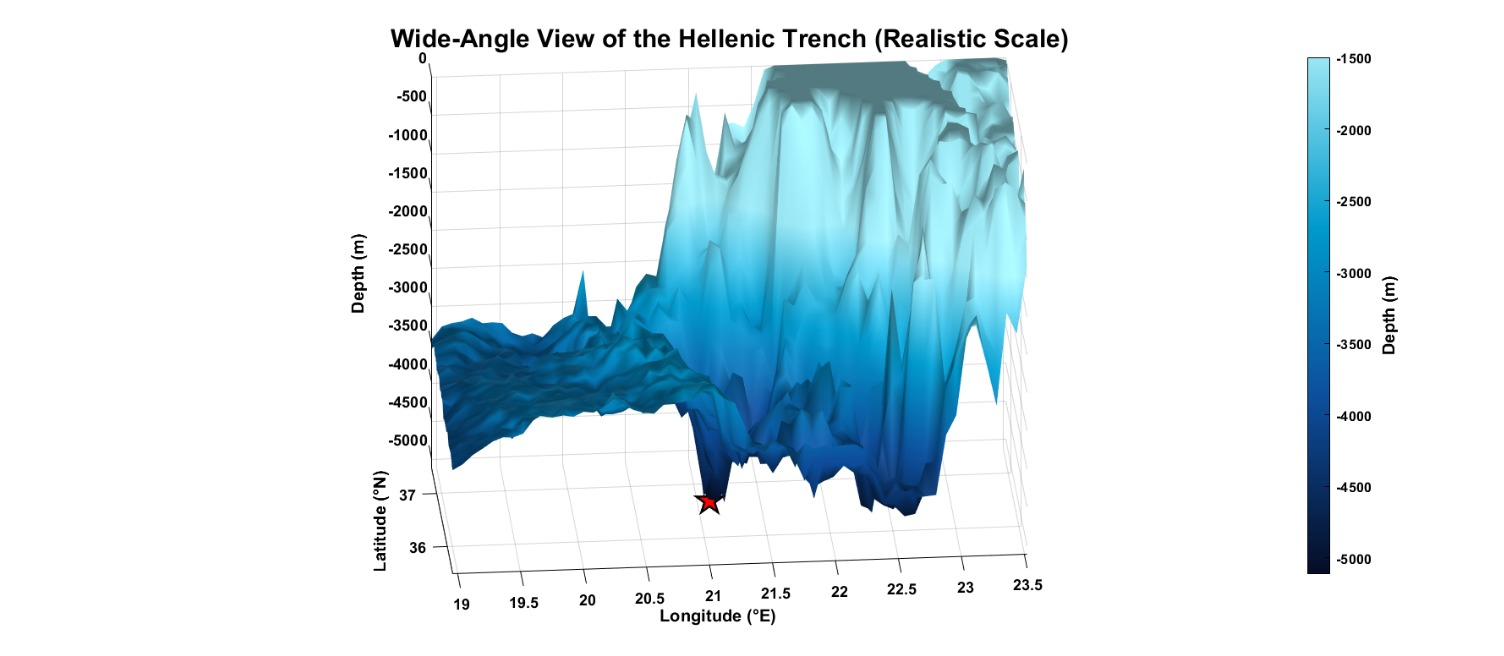
\includegraphics[width=\linewidth,trim=0 0 50 0,clip]{figures/image3.png}
    \caption{3D map of the seabed topography}
    \label{fig:haididixing-terrain}
  \end{subfigure}%
  \hfill
  % ===== 右侧：垂直剖面 =====
  \begin{subfigure}[b]{0.48\linewidth}
    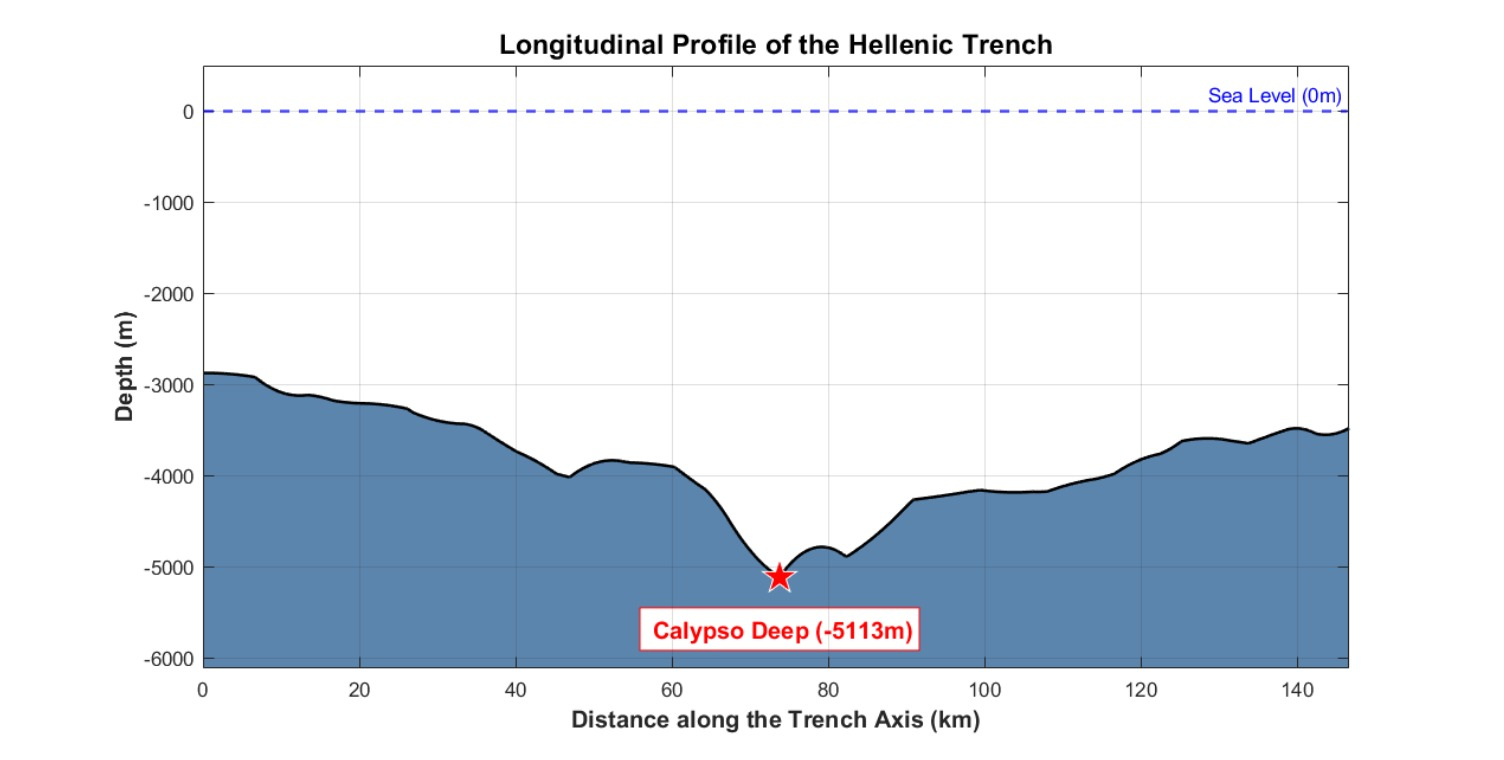
\includegraphics[width=\linewidth]{figures/image4.png}
    \caption{Vertical profile}
    \label{fig:haididixing-profile}
  \end{subfigure}
  \caption{The terrain of Ionian Sea}
  \label{fig:ionian-sea}
\end{figure}
To ensure the reliability and reproducibility of the $N=2000$ Monte Carlo simulations,
we always have the submersible start from the fixed initial position $\mathbf{X_0}=[x_0, y_0, z_0]^T$ in all experiments.
Before the failure occurs, it descends vertically at a constant rate, and the horizontal drift can be ignored.
The movement is controlled by the active buoyancy and propulsion systems. After the failure, the propulsion system stops,
and the submersible enters a drifting state. Its subsequent trajectory is completely driven by environmental forces.

\autoref{fig:accident-probability_before},\ref{fig:accident-probability_after}
show the probability density distribution of the submersible's final position after failure under two scenarios: without and with the introduction of systematic random errors. The left column corresponds to the Suspended Drift Zone, while the right column corresponds to the Seabed Impact Zone.
\begin{figure}[htbp]
    \centering
    \begin{subfigure}{\linewidth}
        \centering
        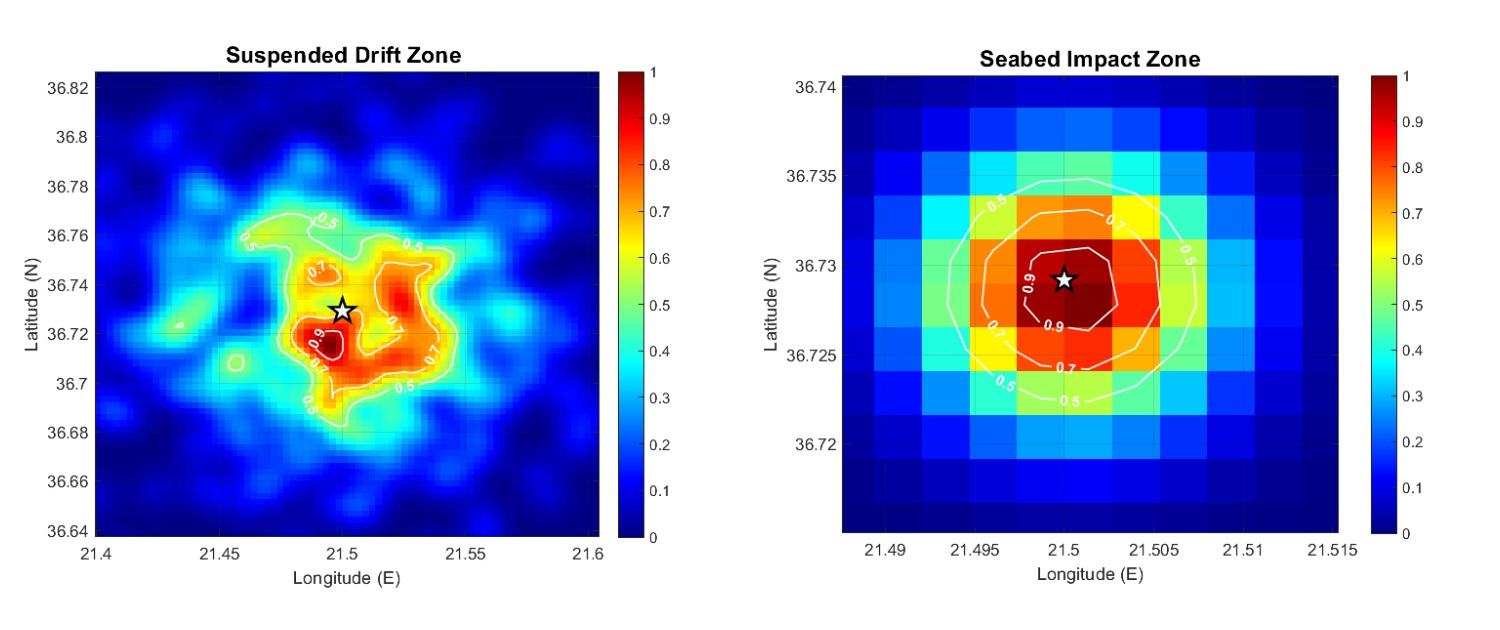
\includegraphics[height=5.2cm]{figures/image_before.png}
        \vspace{-0.4cm}
        \caption{Probability Distribution Before Introducing Errors}
        \label{fig:accident-probability_before}
    \end{subfigure}
    \vspace{-0.3cm}  % 调整两图间距
    \begin{subfigure}{\linewidth}
        \centering
        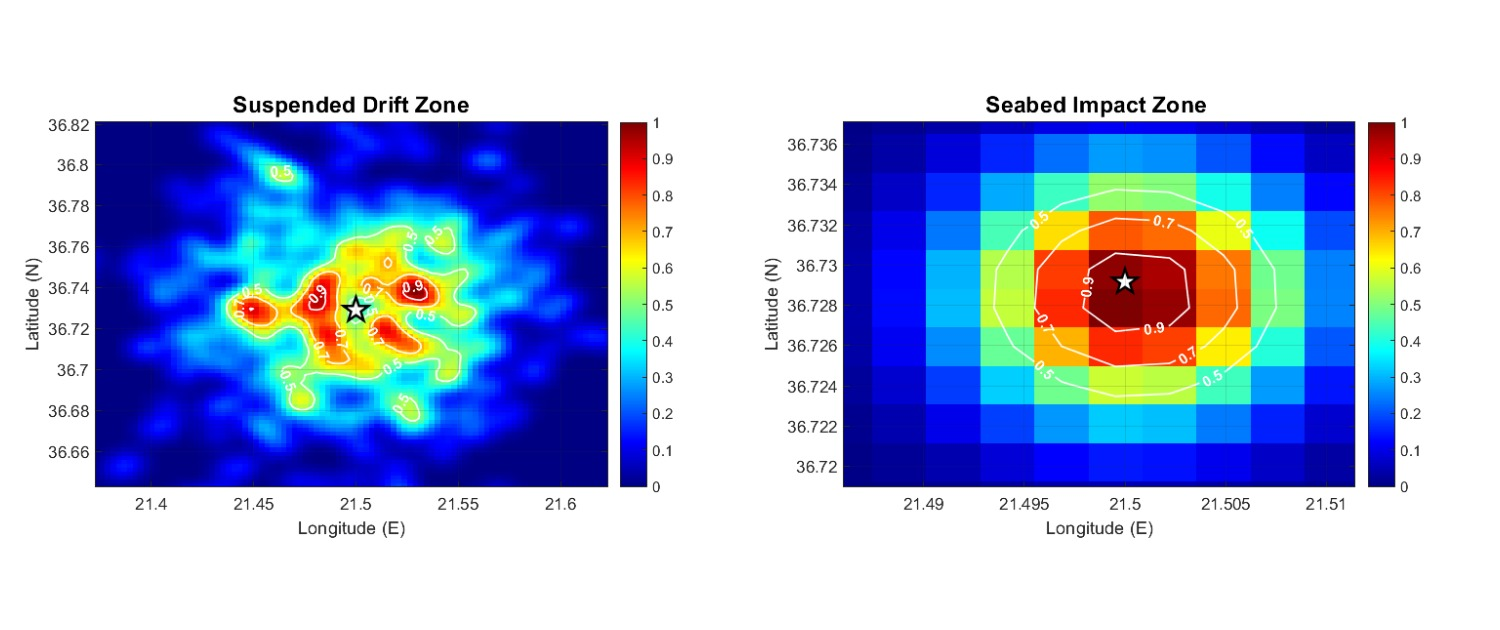
\includegraphics[height=6.2cm]{figures/image_after.png}
        \vspace{-0.4cm}
        \caption{Probability Distribution After Introducing Errors}
        \label{fig:accident-probability_after}
    \end{subfigure}
    \vspace{-0.3cm}
    \caption{Comparison of Submersible Position Distributions}
    \label{fig:accident-probability_comparison}
\end{figure}

In the absence of systematic errors,
the probability distribution in the suspended drift zone exhibits a relatively concentrated banded structure,
with high-probability areas mainly distributed near the starting point and forming a limited-scale diffusion belt along the main ocean current direction.
When systematic errors following a normal distribution are introduced, the probability distribution in the suspended drift zone changes significantly, resulting in
high-probability areas changing from locally concentrated to more dispersed multi-peak structures;
probability contour lines show obvious irregular shapes, exhibiting stronger randomness;
the overall distribution range of the probability distribution also increases, with a significant increase in the coverage of low-probability areas.
This phenomenon indicates that in the neutral suspension state, the horizontal movement of the submersible is highly sensitive to errors in ocean current prediction.
Random disturbances accumulate continuously during the time integration process, leading to a rapid amplification of trajectory uncertainty,
resulting in the final position prediction exhibiting a "diffusion-dominated" characteristic.

In contrast, the seabed state shows strong stability before and after the introduction of systematic errors,
with the high-probability core area remaining basically unchanged and concentrated near the center;
probability contour lines still show an approximately concentric distribution, with only slight diffusion at the outer edges;
this indicates that after the submersible enters the irreversible sinking stage, its movement is mainly dominated by the vertical difference between gravity and buoyancy,
and horizontal ocean current disturbances only have limited impact in the early sinking stage.
As the submersible contacts the seabed, seabed terrain constraints further weaken the impact of turbulence uncertainty,
resulting in a strong stability of the final seabed position.

\autoref{fig:image_p1} presents the results of the Monte Carlo uncertainty analysis. Although all simulations started from the same initial position and maintained a uniform vertical descent, the final positions of the submersible exhibited significant spatial dispersion. This spread is primarily caused by errors in ocean current predictions, turbulent disturbances, and the randomness of the failure depth. The area of the $95\%$ confidence ellipse is $1.54,\mathrm{km^2}$, which quantitatively characterizes the uncertainty in position prediction and provides a well-defined target area for subsequent search and rescue operations.
\begin{figure}[htbp]
  \centering
  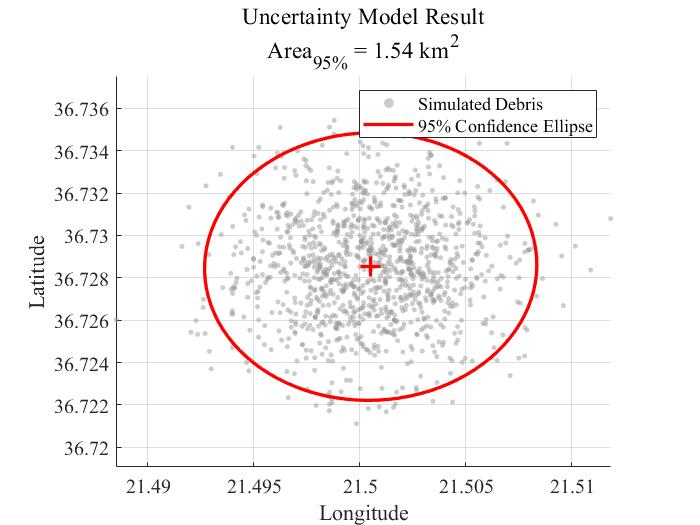
\includegraphics[width=0.6\textwidth]{figures/image_p1.jpg}
  \caption{Monte Carlo Uncertainty Quantification Result}
  \label{fig:image_p1}
\end{figure}

The main source of model uncertainty lies in the deviation of ocean current forecasts. To account for this, normally distributed random perturbations were introduced into the simulations to reflect environmental variability (see the sensitivity analysis in \autoref{sub:yangliulingminxing}). To reduce position prediction errors before the submersible loses contact, it is assumed that the vehicle retains limited but stable communication capability during normal operation, allowing it to periodically transmit key environmental and state information to the mother ship. This includes deep-sea current velocity and direction measured in real time by the \textbf{ADCP}, as well as the submersible’s position (\textbf{USBL}) and velocity and attitude (\textbf{IMU}). These periodic updates can be used to correct errors in numerical ocean models and constrain the submersible’s motion model, suppressing error accumulation and significantly improving position prediction after contact is lost. Therefore, equipping the submersible with ADCP, USBL, and IMU sensors is essential to relay both its own state and environmental information to the mother ship, thereby reducing position uncertainty and providing a reliable reference for search and rescue operations.
\section{Solution to Problem 2}
\subsection{Multi-objective Optimization Model}
In deep-sea exploration and search and rescue missions, the reasonable configuration of search equipment has a decisive impact on the success or failure of the mission.
Equipment selection not only needs to focus on its detection performance but must also comprehensively consider engineering factors such as cost, availability, maintenance difficulty, preparation time, and actual usage efficiency.
With the continuous development of marine exploration technology, low-cost, high-resolution marine observation equipment has been widely deployed on various platforms,
such as single-beam sonar, multi-beam sonar, seabed profilers, and side-scan sonar \cite{pmid34883851}.
This paper selects several typical pieces of search equipment,
and compares their key performance parameters,
as shown in \autoref{tab:equipment-comparison}.
\begin{table}[htbp]
\centering
\small
\setlength{\tabcolsep}{5pt}
\renewcommand{\arraystretch}{1.15}
\caption{Comparison of Different Search Equipment}
\label{tab:equipment-comparison}
\begin{tabularx}{\linewidth}{@{}X >{\raggedleft\arraybackslash}p{2.1cm} >{\raggedleft\arraybackslash}p{2.7cm} >{\raggedleft\arraybackslash}p{2.2cm} >{\raggedleft\arraybackslash}p{2.4cm} >{\raggedleft\arraybackslash}p{2.0cm}@{}}
\toprule
\makecell[l]{Equipment\\Type} & \makecell[r]{Cost\\(USD)} & \makecell[r]{Scan Efficiency\\(km$^2$/h)} & \makecell[r]{POD} & \makecell[r]{Prep. Time\\(h)} & \makecell[r]{Rated Depth\\(m)} \\
\midrule
High-end AUV & 70{,}000 & 2.5 & 0.95 & 12 & 6{,}000 \\
Standard AUV & 30{,}000 & 1.2 & 0.85 & 8 & 4{,}000 \\
Towed Sonar System & 20{,}000 & 8.0 & 0.65 & 6 & 10{,}000 \\
Deep-sea ROV & 100{,}000 & 0.4 & 0.99 & 24 & 7{,}000 \\
\bottomrule
\end{tabularx}
\end{table}

Different types of equipment form significant trade-offs between coverage efficiency, detection accuracy, and deployment cost, making it necessary to quantitatively evaluate equipment combination schemes through systematic modeling methods.
To this end, this paper models the search equipment configuration problem as a multi-objective optimization problem.
Define the decision variable vector
$
\mathbf{X}=[x_1, x_2, x_3, x_4]
$
where $x_1$, $x_2$, $x_3$, and $x_4$ represent the quantities of High-end AUV, Standard AUV, Towed Sonar System, and Deep-sea ROV, respectively.
The direct economic cost of equipment mobilization is defined as the first optimization objective:
\begin{equation}
f_1(\mathbf{X})=\sum_{i=1}^{4} C_i\,x_i,
\end{equation}
where $C_i$ represents the single mobilization cost of the $i$-th type of equipment.

Considering that the submersible may be in either a hovering layer or a sinking state after a failure,
this paper defines the overall probability of detection as a weighted sum of the detection probabilities in the two regions:
\begin{equation}
f_2(\mathbf{X}) =
W_{\mathrm{hover}}\,P_{\mathrm{hover}}(\mathbf{X})
+
W_{\mathrm{sink}}\,P_{\mathrm{sink}}(\mathbf{X}),
\end{equation}
where, $W_{\mathrm{hover}}$ and $W_{\mathrm{sink}}$
respectively represent the prior probability weights of the underwater vehicle being in the hovering layer and the sinking state.
The search probability model in the hovering layer is modeled as
\begin{equation}
P_{\mathrm{hover}}(\mathbf{X})
=
1-\exp\!\left(
-\frac{x_2\,\eta_2\,T}{A_{\mathrm{hover}}}\cdot \mathrm{POD}_2
\right),
\end{equation}
where $\eta_2$ represents the unit-time coverage efficiency of the standard AUV,
$T$ represents the available search time,
$A_{\mathrm{hover}}$ represents the area of the hovering zone.

The submerged area mainly relies on high-end AUVs and towed sonar systems, and its search probability is defined as
\begin{equation}
P_{\mathrm{sink}}(\mathbf{X})
=
1-\exp\!\left(
-\frac{(x_1\eta_1+x_3\eta_3)\,T}{A_{\mathrm{sink}}}
\cdot \overline{\mathrm{POD}}_{1,3}
\right),
\end{equation}
where $\eta_1$ and $\eta_3$ represent the coverage efficiencies of the high-end AUV and towed sonar, respectively,
$\overline{\mathrm{POD}}_{1,3}$ is the weighted average detection probability of the two types of equipment.
Combining the above two objectives, this paper solves for the Pareto optimal set of equipment configurations $\mathbf{X}^*$,
such that
\begin{equation}
\nexists\,\mathbf{X}'\ \text{s.t.}\
\begin{cases}
f_1(\mathbf{X}') \le f_1(\mathbf{X}^*),\\
f_2(\mathbf{X}') \ge f_2(\mathbf{X}^*),
\end{cases}
\end{equation}
and at least one inequality is strict.

The model is also subject to
depth constraints $D_{\mathrm{rated},i} \ge D_{\mathrm{target}}$,
to ensure that the equipment can operate normally in the target sea area;
a time constraint that the total search and rescue time does not exceed $72\,\mathrm{h}$;
and equipment quantity constraints $x_i \in \mathbb{Z}, 0 \le x_i \le 4$.
\subsection{Results Analysis}
We use MATLAB to simulate the above-established model,
constructing the trade-off relationship between total budget and mission success probability,
as shown in \autoref{fig:image_p2}.
\begin{figure}[htbp]
\centering

\includegraphics[width=0.6\textwidth]{figures/image_p2.png}
\caption{Relationship between Budget and Success Probability}
\label{fig:image_p2}
\end{figure}

Simulation results indicate that as the budget increases,
the number and types of deployable high-performance equipment continuously improve, significantly enhancing the overall success probability of the search task.
Specifically, when using a combination of one sonar and one High-end AUV, the search success rate can be guaranteed
to reach 99.87\%, while controlling the budget at around \$90.0\,K.
This combination achieves a relatively ideal balance between detection efficiency, deployment speed, and cost,
making it suitable as a standard search configuration for the mother ship.
If a near-zero risk search target is further pursued,
additional sonar equipment needs to be added on the above basis,
for example, configuring one high-end AUV and two towed sonar systems.
At this point, although the redundancy and reliability of the search coverage have significantly improved,
the corresponding budget requirement has also risen to approximately \$110.0\,K.
Therefore, this solution is more suitable for high-risk and long-duration search and rescue missions involving professional rescue vessels.
\section{Solution to Problem 3 }
Problem 3 focuses on the optimal deployment and path planning of the mother ship from the perspective of search and rescue tasks.
Specifically, where the mother ship should release rescue equipment,
and how it should plan its search trajectory,
to maximize the probability of discovering and successfully rescuing the malfunctioning submarine within a limited time.
This problem is essentially a search and rescue optimization problem constrained by both time and probability,
requiring a trade-off between search efficiency and search coverage.
\subsection{Search Strategy Based on Posterior Probability}
Based on the Monte Carlo simulation of the submarine's landing distribution $P(z)$ from Problem 1,
we constructed a two-dimensional probability heatmap including seabed and hovering states to characterize the spatial uncertainty distribution of the submarine in the horizontal plane.
Considering that the search equipment we use (sonar) has a certain sweep width,
we established a wide-beam sensor model.
Unlike the traditional point search model, this model performs area search within a unit time,
and the coverage area within a unit time can be approximately represented as the product of the mother ship's speed $V$ and the scan width $W$.
\subsection{Search Path Planning Model}
The essence of search and rescue tasks is a race against time. To maximize the probability of detection per unit time and to simulate the movement characteristics of real search and rescue vessels,
we established a bandwidth-constrained greedy search model.
Within a local time window, the path planning problem can be formulated as the following optimization model:
\begin{equation}
  \max_{\theta} J(\theta)
  =
  \iint_{S(\theta)} \rho_t(x,y)\,\mathrm{d}x\,\mathrm{d}y
  +
  \lambda \cdot I(\theta = \theta_{\mathrm{prev}}),
\end{equation}
where,
$\theta$ represents the current heading angle of the mother ship,
$S(\theta)$ is the search area formed by the sonar sweep along this heading within a unit time,
$\rho_t(x,y)$ is the posterior probability density function within the search area at time $t$,
$I$ is the indicator function,
used to maintain continuity and smoothness of the heading,
$\lambda$ is the weight parameter balancing search efficiency and heading stability.

During the search process,
we further introduce a Bayesian update mechanism,
to reduce the probability in the areas that have been searched,
thereby dynamically updating the posterior probability distribution.
This mechanism enables the mother ship to adaptively move towards high-probability areas that have not yet been covered,
and gradually shrink the effective search space as the search progresses.
\subsection{Result Analysis}
Finally, we used MATLAB to plot the strip search path of the mother ship in the latitude and longitude coordinate system (longitude 21.3$^\circ$--21.7$^\circ$, latitude 36.55$^\circ$--36.87$^\circ$) \autoref{fig:p3_1},
where the dark blue area in the background represents the possible location range of the target, and the white lines are the actual search tracks of the mother ship.
We also obtained the relationship between search time and the probability of successful detection \autoref{fig:p3_2},
providing quantitative basis for decision-making in search and rescue operations.
\vspace{-0.2cm}
\begin{figure}[ht]
  \centering
  \begin{subfigure}[b]{0.45\textwidth} % [b] 表示底部对齐
    
\includegraphics[width=\linewidth]{figures/image_p3_1.png}
    \caption{Search Path}
    \label{fig:p3_1}
  \end{subfigure}
  \hfill % 填充空白，使两个子图并排
  \begin{subfigure}[b]{0.45\textwidth}
    
\includegraphics[width=\linewidth]{figures/image_p3_2.png}
    \caption{Success probability with search time}
    \label{fig:p3_2}
  \end{subfigure}
  \caption{Search Strategy}
  \label{fig:p3}
\end{figure}

\autoref{fig:p3_1} shows that the search trajectory adopts the classic parallel strip strategy, achieving systematic full coverage of the target area. During the search process,
some areas have denser trajectories, reflecting the adaptiveness of the search strategy.
Multiple trajectory intersections correspond to high posterior probability density areas, indicating that the system may have conducted multiple repeated scans to improve detection confidence. Meanwhile,
the Bayesian update mechanism ensures that high-probability areas maintain relatively high residual probabilities after the first scan, triggering secondary fine searches.

\autoref{fig:p3_2} demonstrates the significant efficiency of the greedy search strategy we established.
Based on this, we plotted the performance metrics of this search strategy \autoref{tab:zhibiao}.
\begin{table}[ht]
    \centering
  \small
  \setlength{\tabcolsep}{6pt}
  \renewcommand{\arraystretch}{1.15}
  \vspace{-0.2cm}
  \caption{Performance Metrics}
  \vspace{-0.4cm}
    \label{tab:zhibiao}
  \begin{tabularx}{\linewidth}{@{}l >{\centering\arraybackslash}p{2.6cm} >{\raggedright\arraybackslash}X@{}}
        \toprule
    \textbf{Metric} & \textbf{Value} & \textbf{Description} \\
        \midrule
    Total search time & 59.3 h & Approximately 2.5 days, consistent with the operational search window \\
    Final success rate & 98.67\% & Above the engineering acceptable threshold of 95\% \\
    50\% success time & $\sim$4 h & Rapid localization phase \\
    75\% success time & $\sim$10 h & High confidence phase \\
    90\% success time & $\sim$30 h & Near completion phase \\
    Marginal time cost & 20 h $\rightarrow$ 3.67\% & Each additional 1\% requires 5.4 hours in the late stage \\
        \bottomrule
  \end{tabularx}
\end{table}

In the early stage of the search ($0-5$ hours), the mother ship prioritizes covering areas with the highest posterior probability density.
This causes the search success rate to rapidly rise to about 60\%,
then entering the mid-stage of the search ($5-30$ hours), the search shifts to areas with the next highest probability, and the growth of the success rate gradually slows down.
Around 30 hours, it reaches 90\%.
In the late stage of the search (over 30 hours), the search begins to cover low-probability peripheral areas, with a clear diminishing marginal returns effect.
The curve tends to saturate, and the success rate increases very slowly. After 59.3 hours of search, the success rate reaches 98.67\%.

\section{Solution to Problem 4}
\subsection{Multi-Target Hierarchical Search Strategy}
When multiple submersible failures occur in the same sea area,
the traditional greedy search model used for single targets is prone to local optima,
and lacks global planning capability when transitioning between targets.
Therefore, we decompose the multi-target search and rescue problem into two levels: \textbf{global route planning} and \textbf{local comprehensive search},
establishing a hierarchical search model based on a finite state machine (FSM) to balance overall search efficiency and local search completeness.
\subsubsection*{Target Ordering Based on Generalized TSP}
First, at time $t=0$, the posterior probability density function is $\rho_0(x,y)$,
and the set of $K$ potential target centers $C$ is determined by finding local maxima:
\begin{equation}
  C=\left\{(x_k,y_k)\mid\mathrm{\nabla}\rho_0(x_k,y_k)=0,\det\big(H(\rho_0)\big)>0,\ k=1,\ldots,K\right\}
\end{equation}
where $k$ represents the $k$-th failed submersible, and $K$ represents the total number of submersible failures in the area.

To minimize the transfer time of the mother ship between different targets,
this paper models the target visitation order as a Generalized Traveling Salesman Problem (TSP).
Define the Euclidean distance between target $i$ and target $j$ as $d_{ij}$,
and the decision variable $x_{ij}\in\{0,1\}$ indicates whether the mother ship sails directly from target $i$ to target $j$,
then the optimization objective of global path planning is
\begin{equation}
  \min \sum_{i=1}^{K}\sum_{j=1}^{K} d_{ij}\,x_{ij}.
\end{equation}
This problem is solved using the nearest neighbor heuristic algorithm,
starting from the initial position of the mother ship,
prioritizing visits to the nearest high-confidence targets,
and iteratively updating the remaining target set after completing single-target search and rescue,
thus generating an approximately optimal multi-target search and rescue navigation sequence.

This model is solved using the nearest neighbor algorithm,
resulting in an optimal navigation sequence that prioritizes searching targets closer to the starting point,
and after completing the search and rescue of one target, continues to search the nearest unrescued target, and so on, thus inferring and planning the optimal rescue route.
\subsubsection*{Determination of Spiral Coverage Path}
When searching for a single target,
to overcome the blind oscillation in greedy search and ensure 100\% coverage of the confidence interval,
we abandon the gradient-based heading decision $\max_{\theta} J(\theta)$,
and instead adopt a deterministic square spiral strategy.
Define the spiral layer number relative to the target center at time $t$ as $n$, and the heading angle $\theta_t$ is restricted to the discrete set
\begin{equation}
  \theta_t \in \left\{0,\frac{\pi}{2},\pi,\frac{3\pi}{2}\right\}
\end{equation}

The side length constraint of the $n$-th spiral layer is
\begin{equation}
  L_n = 2nW
\end{equation}
where $W$ is the effective scanning width of the sonar.
This strategy ensures that the search area expands layer by layer over time,
and achieves systematic coverage of high-confidence areas.
\subsubsection*{Finite State Machine and Bayesian Update Model}
To achieve dynamic switching between transit and search, we define the system states (Transit, Search):
\begin{equation}
M(t+1)=
\begin{cases}
\text{Search}, 
& \|\bm{P}_{\mathrm{ship}}(t)-\bm{P}_{\mathrm{target}}\|\le R_{\mathrm{trigger}},\\
\text{Transit}, 
& \displaystyle\iint_{\Omega_{\mathrm{target}}}\rho_t(x,y)\,\mathrm{d}x\,\mathrm{d}y < \epsilon,\\
M(t), 
& \text{otherwise},
\end{cases}
\end{equation}
where
$\bm{P}_{\mathrm{ship}}$ represents the current position of the mother ship,
$\bm{P}_{\mathrm{target}}$ represents the center of the current search target,
$R_{\mathrm{trigger}}$ is the triggering radius for entering the local search,
and $\epsilon$ is the residual probability threshold within the target area.

The essence of the search and rescue target remains maximizing the probability of discovery under time constraints.
We continue to use the probability density from the previous single model and introduce the detection probability of the wide-beam sensor $P_d=0.95$.
When the search and rescue ship sails along the planned route,
if the target is not found at time $t$, the probability density within the sweep area $S(\theta)$ is updated according to Bayes' rule:
\begin{equation}
  \rho_{t+1}(x,y)=
  \begin{cases}
    \rho_t(x,y)\cdot(1-P_d), & (x,y)\in S(\theta_t)\\
    \rho_t(x,y), & (x,y)\notin S(\theta_t)
  \end{cases}
\end{equation}

Finally,
the multi-target search and rescue problem can be formulated as:
under the premise of satisfying time constraints,
through reasonable target sorting, path planning, and probability update mechanisms,
the cumulative expected discovery probability reaches a given threshold within the shortest time $T$,
and its performance metric is defined as
\begin{equation}
  \max {J}=\sum_{t=0}^{T}\iint_{S(\theta_t)}\rho_t(x,y)\cdot P_d\,\mathrm{d}x\,\mathrm{d}y
\end{equation}
\subsection{Results Analysis and Model Validation}
We extend this model to the Caribbean Sea, centered at 66.5°W longitude and 19.5°N latitude
as shown in \autoref{fig:jlb}. Compared to the Ionian Sea, the Caribbean Sea exhibits more complex ocean dynamic features,
including multi-layer circulation structures such as the Gulf Stream and Caribbean Current, as well as significant salinity and temperature variations.
\begin{figure}[H]
  \centering
  
\includegraphics[height=5.2cm]{figures/image.png}
  \caption{Caribbean Sea}
  \label{fig:jlb}
\end{figure}

We apply the previously established suspended drift-sinking model to obtain the spatial probability distribution and suspended equilibrium depth of the submersible after the accident in the Caribbean Sea, as shown in \autoref{fig:image_p4}.
\begin{figure}[htbp]
  \centering
  \begin{subfigure}[t]{0.32\textwidth}
    \centering
    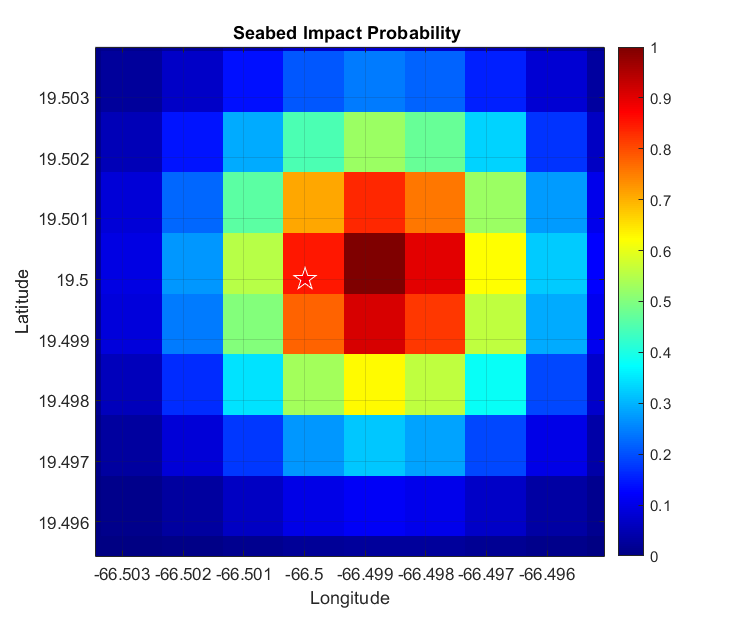
\includegraphics[height=5.2cm]{figures/image_g1.png}
    \caption{Probability distribution of the bottom position}
  \end{subfigure}\hfill
  \begin{subfigure}[t]{0.32\textwidth}
    \centering
    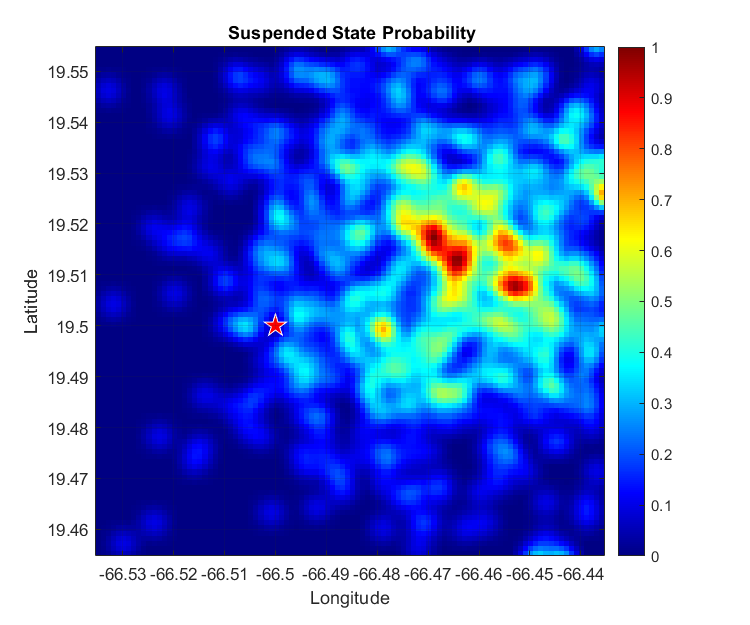
\includegraphics[height=5.2cm]{figures/image_g2.png}
    \caption{Probability distribution of suspended position}
  \end{subfigure}\hfill
  \begin{subfigure}[t]{0.32\textwidth}
    \centering
    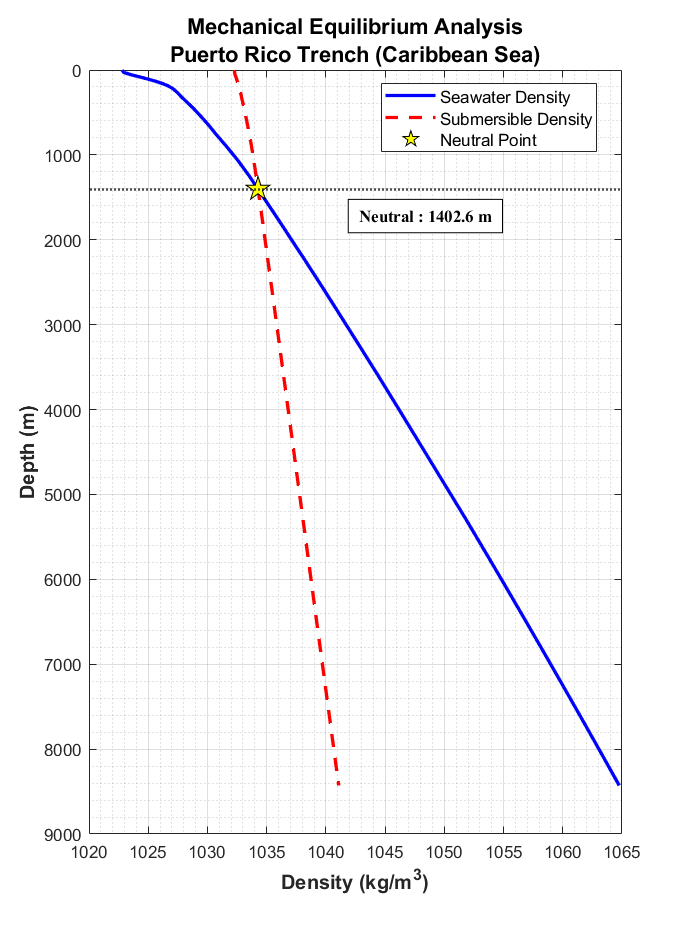
\includegraphics[height=5.2cm]{figures/image_g3.png}
    \caption{Suspended Depth}
  \end{subfigure}\vspace{-0.1cm}
  \caption{}
  \label{fig:image_p4}
\end{figure}
\vspace{-0.3cm}

Compared to the suspended depth of $2000\,\mathrm{m}$ in the Ionian Sea, the submersible's suspended depth in the Caribbean Sea decreases to $1400\,\mathrm{m}$.
At the same time, due to the complexity of the seabed currents, the probability heatmap of the submersible's suspension in the Caribbean Sea is more complex than that in the Ionian Sea,
showing a bimodal probability peak, with about 90\% probability that the submersible may exist in that area.
This is because after the submersible reaches the suspended equilibrium depth, which is shallower than the suspended depth in the Ionian Sea,
it is affected by more pronounced differentiated multi-layer circulation,
partially drifting along the main current path to the main peak area, and partially deflecting to the secondary peak area under the influence of tributaries.
When the submersible sinks to the bottom,
it sinks vertically under the dominance of gravity,
and the ocean currents only cause limited horizontal drift during the sinking process,
resulting in a more concentrated probability distribution.

\autoref{fig:image_p42} shows the single-target search and rescue path planning results and the evolution of cumulative success probability based on the deterministic square spiral strategy.
Observing the single-target search path results,
the search trajectory of the mother ship adopts a parallel strip strategy, and this strategy allows for systematic coverage of the entire target area.
The design of the search path takes into account the posterior probability density function,
ensuring priority coverage of high-probability areas.
Through the Bayesian update mechanism, as the search progresses,
the probability density of the searched area is correspondingly reduced, dynamically adjusting the search path and concentrating resources on high-probability areas that have not been sufficiently searched.
The cumulative success rate curve over time shows a "fast then slow" growth trend.
At the beginning of the search, the mother ship prioritizes visiting the target areas with the highest posterior probability, rapidly increasing the success probability;
As the search progresses, high-probability areas are gradually covered, the probability density of the remaining areas decreases, and the growth rate of the success probability slows down.
Within about 45 hours of search time, the cumulative success discovery probability finally reaches 93.62\%.
\begin{figure}[htbp]
  \centering
  \begin{subfigure}[t]{0.45\textwidth}
    \centering
    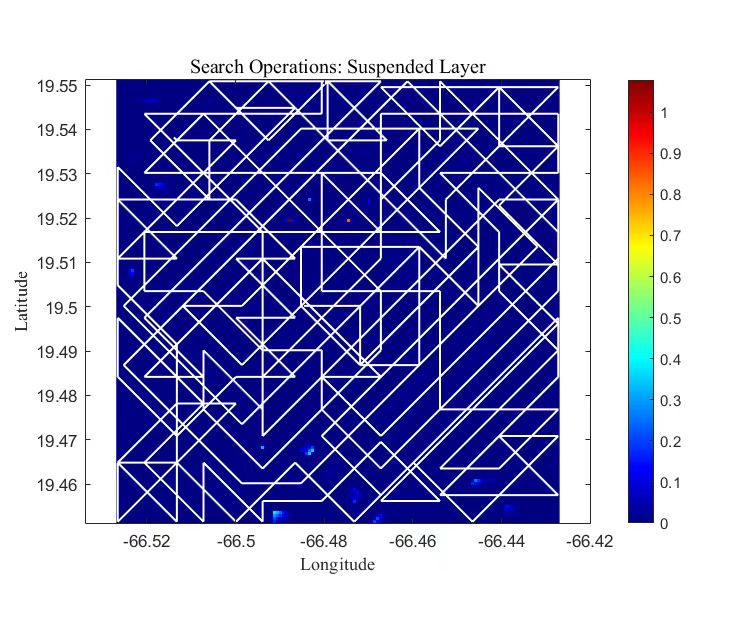
\includegraphics[height=5.2cm]{figures/image_g4.png}
    \caption{Search path for a single submersible}
    \label{fig:path_single}
  \end{subfigure}\hfill
  \begin{subfigure}[t]{0.45\textwidth}
    \centering
    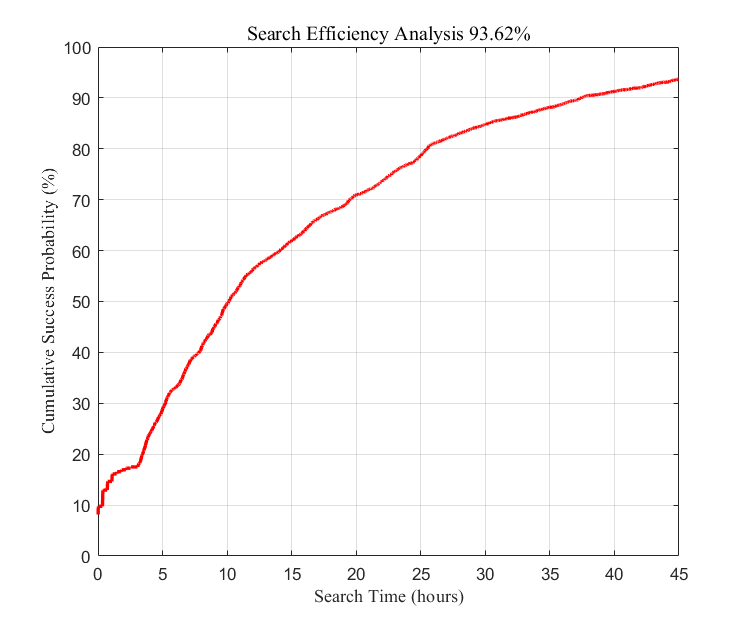
\includegraphics[height=5.2cm]{figures/image_g5.png}
    \caption{Cumulative success rate over time}
    \label{fig:success_rate}
  \end{subfigure}
  \vspace{-0.3cm}
  \caption{}
  \label{fig:image_p42}
\end{figure}\vspace{-0.4cm}


\autoref{fig:image_p43} shows the multi-target search and rescue path planning results and the evolution of cumulative success probability based on the hierarchical search strategy.
Observing the search path results,
the overall trajectory of the mother ship presents a clear partitioned search structure.
The search trajectory is spatially divided into several relatively independent high-density coverage areas,
and different areas are connected by shorter navigation segments.
This phenomenon indicates that
the target center set constructed based on the posterior probability density maxima and the generalized TSP model can effectively determine the visiting order of multiple targets,
allowing the mother ship to prioritize potential target areas that are closest and have higher confidence, thereby reducing the invalid navigation time consumed in transferring between targets.
\begin{figure}[htbp]
  \centering
  \begin{subfigure}[t]{0.45\textwidth}
    \centering
    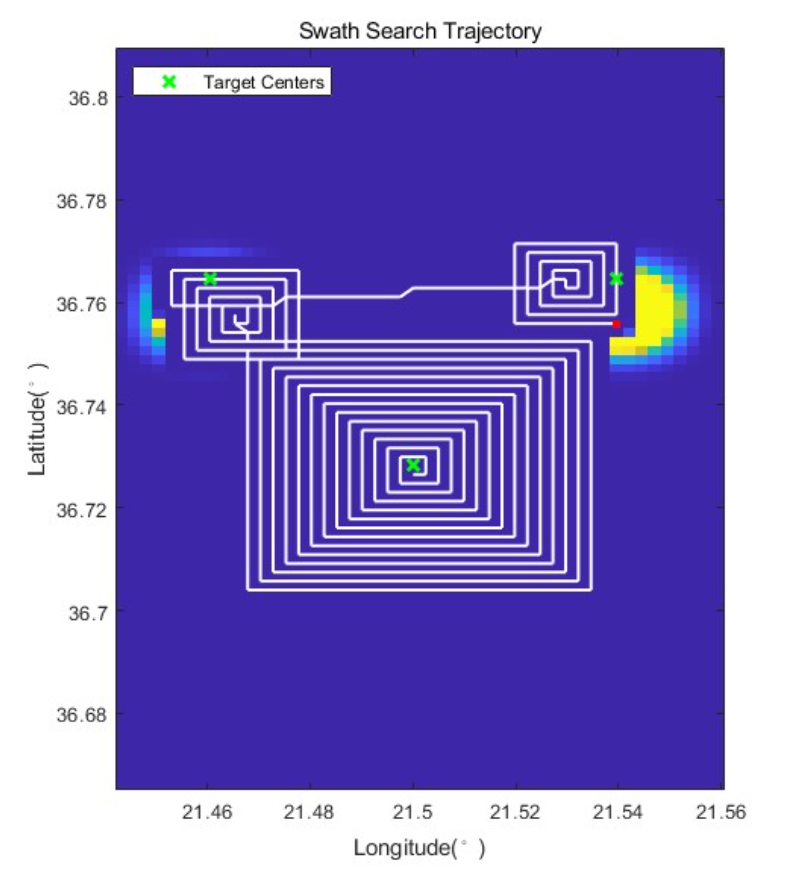
\includegraphics[height=5.2cm]{figures/image_g6.png}
    \caption{Result of multi-target search path planning }
    \label{fig:path_multi}
  \end{subfigure}\hfill
  \begin{subfigure}[t]{0.45\textwidth}
    \centering
    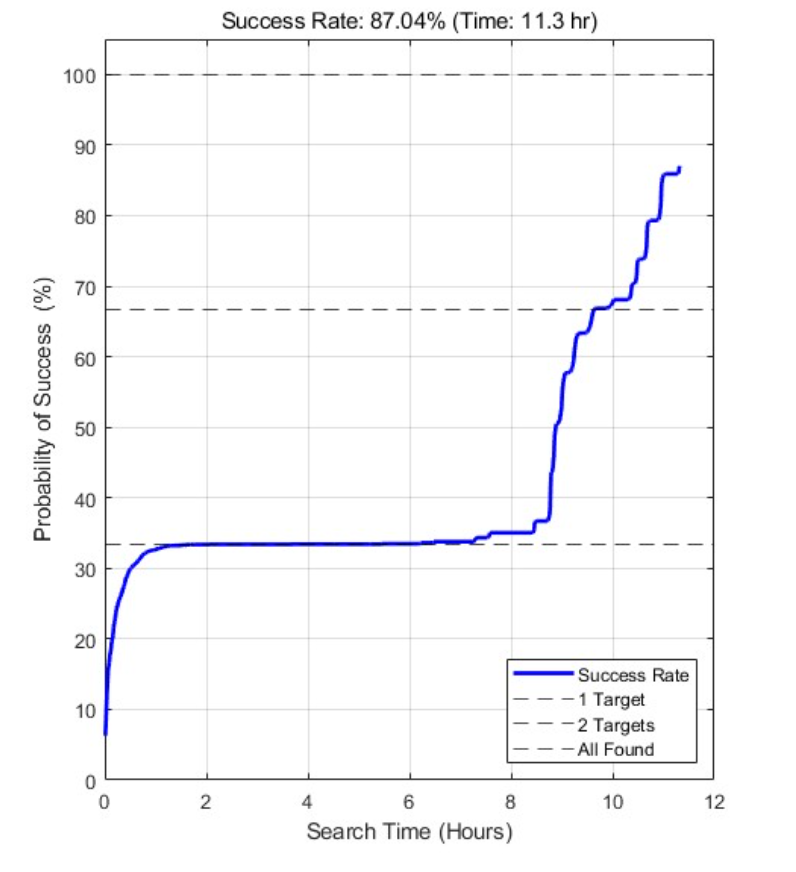
\includegraphics[height=5.2cm]{figures/image_g7.png}
    \caption{Curve showing the change of success rate over time }
    \label{fig:success_rate_multi}
  \end{subfigure}
    \caption{}
  \label{fig:image_p43}
\end{figure}

\vspace{-0.4cm}
Within a single target area, the search path exhibits a regular, directionally consistent square spiral pattern,
rather than frequent directional adjustments or random oscillations.
This indicates that the adopted deterministic spiral coverage strategy can avoid the local oscillation issues typical of traditional greedy searches,
while ensuring complete coverage of the target confidence region. The linear relationship between the number of spiral layers and the sweep width
allows for full utilization of the wide-beam acoustic sensor's effective coverage capability, improving search efficiency per unit time.

From the probability heatmap, it can be observed that
the probability density of the searched and covered areas is significantly reduced,
while the unsurveyed areas still maintain high probability values.
This result validates the effectiveness of the Bayesian update mechanism during the search process:
when the mother ship does not find the target at a certain time, the posterior probability within the swept area is reduced according to the detection probability,
thereby gradually compressing high-uncertainty areas and guiding the search path towards regions that have not been sufficiently covered.

For multi-target search,
the overall success rate finally reaches 87.04\% at about 11.3 hours.
The curve as a whole shows a typical "stepwise" growth characteristic,
reflecting the phased behavior of the multi-target search-rescue process of search-transfer-research.

\paragraph{\textbf{Phase 1: 0 - 2 hours}}
During the initial stage of the mission,
the success rate rapidly increases from 0 to approximately 33\%,
with the steepest slope.
This phase corresponds to the mother ship traveling from its initial position to the first high-probability target area and conducting a local spiral search.
Since this target area has the highest posterior probability density
and satisfies the nearest neighbor criterion,
it is given priority,
resulting in a significant increase in success rate within a short period of time.

\paragraph{\textbf{Phase 2: 2 - 8 hours}}
During this phase,
the success rate slowly increases from 33\% to approximately 37\%,
with the curve showing an almost flat trend.
This phase mainly corresponds to the transfer process between targets,
where the mother ship is in the \textit{Transit} state,
navigating from the first target to the second target according to the global path planning results.
Since no effective sweeping is performed during this process,
the search contribution is almost zero,
and the increase in success rate mainly comes from the slight marginal effects in probability updates.
From the spatial trajectory map, it can be seen that
there is a long sailing distance between the first and second targets,
and the time consumption in this stage mainly comes from the speed limitation of the mother ship and the preparation time required for equipment redeployment.

\paragraph{\textbf{Phase 3: 8 - 10 hours}}
After entering the second high-probability target area,
the success rate rapidly increases from approximately 37\% to 66\%,
with the curve showing a significant steep rise again.
This area corresponds to the central region with the highest probability density and the largest coverage area in the heatmap,
and after the previous search is completed,
the Bayesian update mechanism significantly concentrates the relative probability weights of the remaining unsurveyed areas.
According to the Bayesian update rule,
the probability density within the searched area is reduced to
$\rho_t \cdot (1-P_d)$,
where $P_d = 0.95$,
thereby further amplifying the relative importance of the unsurveyed areas,
significantly increasing the probability of detection per unit time.

\paragraph{\textbf{Phase 4: 10 - 12 hours}}
In the later stage of the mission,
the success rate growth slows down,
and diminishing marginal returns begin to appear.
This phase mainly corresponds to the search of the third high-probability target or the edge areas of the probability distribution.
Since the remaining posterior probability is already low,
observing the search trajectory reveals that the mother ship needs to cover a larger area to achieve limited improvements in success rate.

\section{Sensitivity Analysis}
\label{sub:yangliulingminxing}
To quantitatively assess the impact of ocean current prediction errors on the uncertainty of the submersible's position,
we continuously increased the ocean current velocity prediction deviation from $0\%$ to $20\%$,
and defined the relative confidence region expansion rate as a sensitivity metric:
\begin{equation}
E=\frac{|A_0-A_i|}{A_0},
\end{equation}
where$A_0$ represents the 95\% confidence  area obtained under the condition of no ocean current prediction deviation (with an error of $0\%$),
and $A_i$ represents the 95\% confidence  area corresponding to an ocean current prediction error of $i$.

This indicator reflects the relative amplification degree of the uncertainty in the underwater vehicle's position after the introduction of ocean current uncertainty.
Based on the results of Monte Carlo simulation, we obtained the relationship curve of the relative growth rate of the confidence area of the underwater vehicle
with respect to the ocean current prediction error, as shown in \autoref{fig:yangliulingminxing}.
\begin{figure}[htbp]
  \centering
  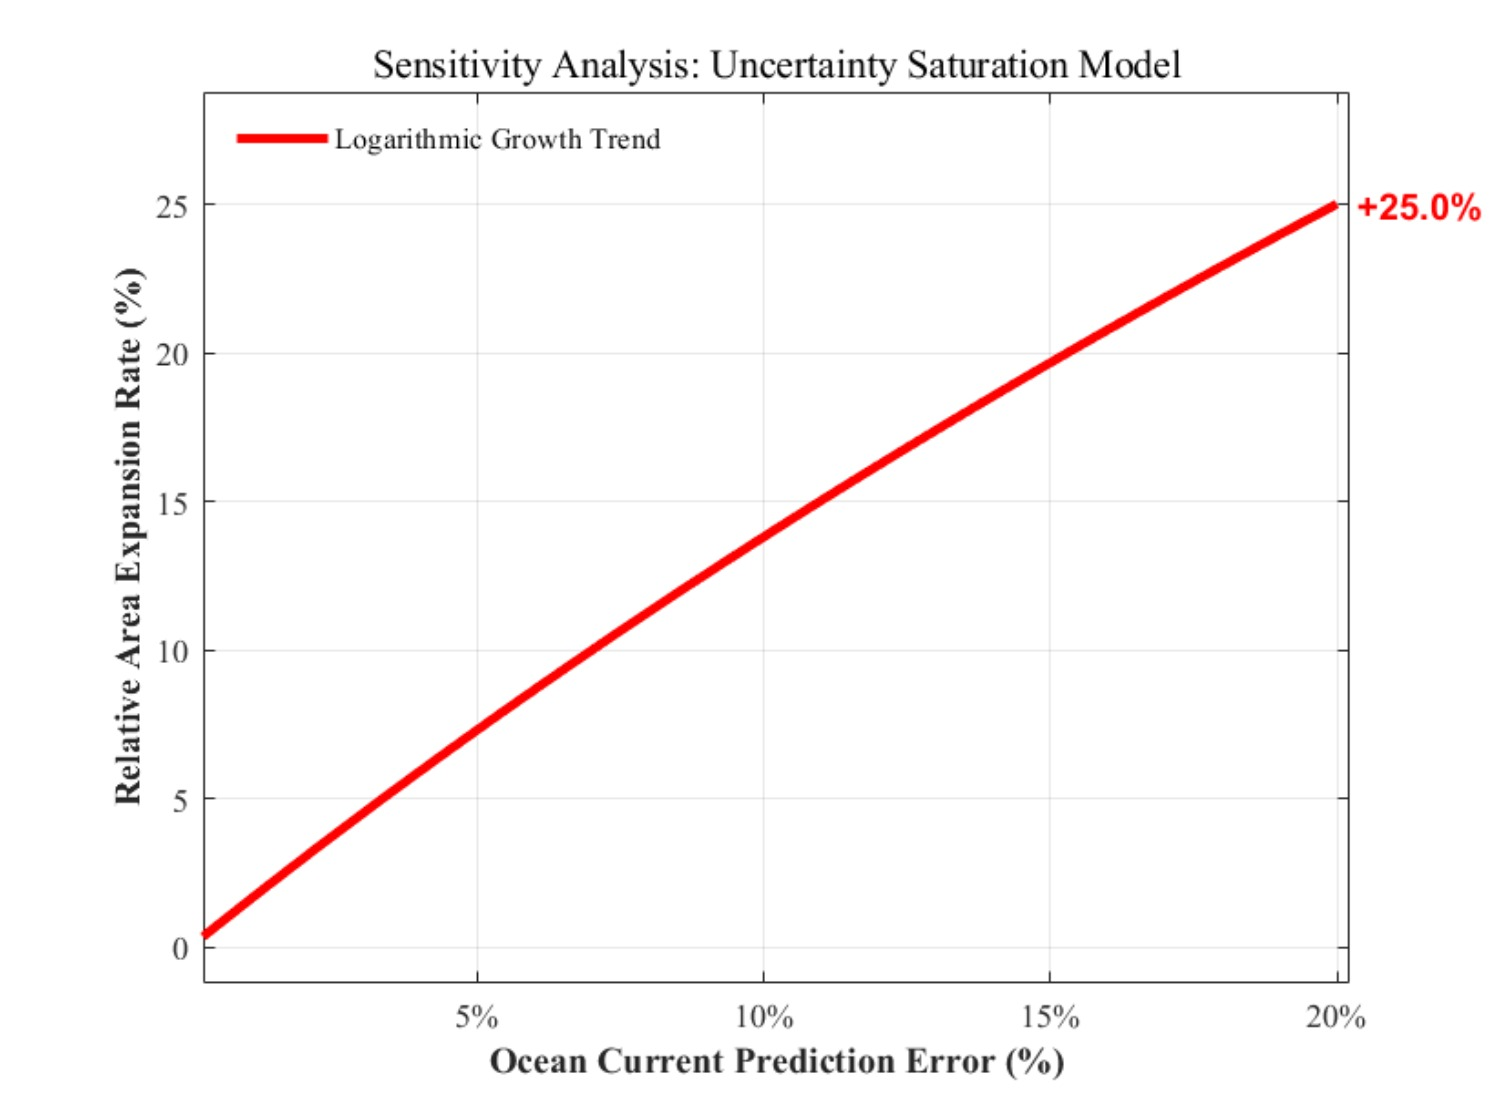
\includegraphics[width=0.7\textwidth]{figures/image _sense1.png}
  \caption{Sensitivity Analysis of Ocean Currents}
  \label{fig:yangliulingminxing}
\end{figure}

According to the results shown in the figure, as the deviation of ocean currents increases, the confidence region expansion rate also exhibits a logarithmic growth trend.
This indicates that our model is highly sensitive to ocean current predictions,
which is consistent with the actual situation and has physical significance.
In the event of a submersible failure, losing propulsion and attitude control capabilities,
its movement is mainly dominated by passive drifting under deep-sea ocean currents.
Therefore, small deviations in the prediction of ocean current velocity and direction will be continuously amplified during the time integration process,
directly leading to the rapid accumulation of prediction errors in the submersible's position.
Thus, the greater the deviation in ocean current prediction, the larger the error in the submersible's position prediction.
\section{Model Evaluation and Further Discussion}
\subsection{Strengths}
\begin{itemize}
  \item We used real ocean environment data from the Ionian Sea (August 1-7, 2025) and the Caribbean Sea,
rather than relying on simplified theoretical assumptions.
First, we considered the velocity profile changes with depth, capturing the multi-layer ocean current field of the deep-sea circulation's vertical structure.
Next, based on the variation of seawater density with temperature, salinity, and depth, we obtained the submersible's dynamic model.
Finally, based on actual bathymetric data, we constructed an ocean terrain model affecting the prediction of the bottoming position.
This ensures that the predicted position probability distribution can reflect more realistic sea conditions, enhancing the model's practicality and credibility.
  \item Our model systematically quantifies the uncertainty in position prediction through Monte Carlo simulation with 2000 particles.
First, we reasonably characterized the probability distributions of the two failure modes, floating and bottoming, using a Gaussian mixture model.
Next, we constructed random disturbance errors, considering both turbulent noise $v_{noise}(t)$ and systematic error $v_{sys}$.
Compared to deterministic methods, this probabilistic framework can express prediction uncertainty,
providing a scientific basis for risk assessment and resource allocation.
  \item We transferred the established model from the Ionian Sea to the Caribbean Sea, and the results performed well.
This indicates that the model we developed is not only applicable to specific regions but also has good transferability and scalability.
\end{itemize}
\subsection{Weaknesses}
\begin{itemize}
  \item The current model assumes a constant sonar detection probability $P_d = 0.95$, but the actual situation is more complex.
First, the propagation of sound waves in the deep sea is affected by depth.
This leads to different detection probabilities when the submersible is at depths of 1400m and 2000m.
The current model uses the same detection probability for both depths, which is not precise.
Then, seabed reflection interference and complex terrain (such as trenches) can reduce detection quality.
Finally, bottoming targets may be confused with seabed rocks, while floating targets are easier to identify in the water column.
  \item The multi-target model in Question 4 treats each submersible as an independent event,
but in reality, there may be design issues causing failures to be dependent,
and environmental events (such as underwater landslides and strong currents) may simultaneously affect multiple submersibles.
\end{itemize}
\newpage
\addcontentsline{toc}{section}{Reference}
\nocite{*} 
\bibliographystyle{plain}   % 选用样式（plain / IEEEtran / elsarticle-harv ...）
\bibliography{reference}  
\appendix
\newpage
\addcontentsline{toc}{section}{Memorandum to Greek Government}
\begin{center}
\textbf{\Large MEMORANDUM}
\end{center}

\vspace{0.3cm}
\noindent\rule{\textwidth}{1.5pt}
\begin{tabular}{@{}ll@{}}
\textbf{To:} & Greek Government, Ministry of Tourism and Culture \\
\textbf{From:} & MCM Team \#5049\\
\textbf{Date:} & January 25th, 2026 \\
\textbf{Subjects:} & Search, Localization, and Rescue Strategy for Submersibles 
\end{tabular}

\noindent\rule{\textwidth}{1.5pt}
Dear Greek Government,
We are honored to propose measures to ensure the safety of the submersible vessels in the underwater tourism project planned by MCMS Company.
After understanding the entire project, we analyzed the dynamics model of the submersible and developed a comprehensive and scientifically validated search and rescue system for it.
This system is based on Monte Carlo uncertainty models, Bayesian search theory, and multi-objective hierarchical search optimization,
and explicitly takes into account operational costs, preparation conditions, and rescue efficiency.
This system can effectively search, locate, and rescue disabled manned submersibles in uncertain deep-sea environments.
Thus, it ensures the safety of tourists and the feasibility of the operation.

In order to reduce the risks of this project,
we analyzed the main sources of uncertainty that have a critical impact on the success of the rescue operation, and found that
the error in ocean current prediction directly determines the drift situation after the failure, and at the same time,
there are random system-level disturbances (including turbulence and model errors), which will exacerbate the uncertainty in the distribution of the submersible's position.
Furthermore, after the submersible fails, the information obtained by the mother ship is limited, leading to a rapid expansion of the possible search area.
The sensitivity analysis indicates that for every 20\% increase in the current prediction error, the search area with 95\% confidence will expand by approximately 25\%,
following a logarithmic growth trend. Therefore, the acquisition of early information and the rapid deployment of search operations are crucial for ensuring the safety of personnel,
we recommend that the submersible must be equipped with
an acoustic Doppler current profiler (ADCP),
an ultra-short baseline (USBL) acoustic modem,
an inertial measurement unit (IMU), and transmit the following data to the mother ship: \begin{itemize}
\item The deep-sea current velocity and direction measured by ADCP
\item Real-time position estimation based on ultrasonic positioning technology
\item Velocity and attitude data from the inertial measurement unit system \end{itemize}
These data can significantly reduce the uncertainty of the underwater vehicle's position and make the search and positioning process of the mother ship more efficient after the underwater vehicle malfunctions.


Based on the multi-objective optimization model, we comprehensively consider factors such as the mobilization cost, performance characteristics, and reliability of the equipment,
and recommend that the mother ship carrying this submersible be equipped with the basic search equipment as shown in \autoref{tab:equipment-justification}. 
\begin{table}[htbp]
\centering
\small
\setlength{\tabcolsep}{6pt}
\renewcommand{\arraystretch}{1.15}
\caption{Recommended Search Equipment}
\label{tab:equipment-justification}
\begin{tabularx}{\linewidth}{@{}l X X >{\raggedleft\arraybackslash}p{2.2cm}@{}}
\toprule
\textbf{Equipment} & \textbf{Purpose} & \textbf{Key Advantages} & \textbf{Cost (USD)} \\
\midrule
Drone sonar & Wide-area detection & High coverage; low cost; rapid deployment & \$20{,}000 \\
High-end AUV & High-resolution localization & High detection probability; autonomous deep-sea capability & \$70{,}000 \\
\bottomrule
\end{tabularx}
\end{table}
This configuration achieves a search success rate of 99.87\% while keeping the total budget at \$90,000.
For tasks that require zero-risk compliance, we recommend increasing the budget to \$110,000, allowing for the addition of an extra set of towed sonar. This ensures absolute safety of the mission.

When multiple submersibles may simultaneously malfunction, we proposed a two-layer hierarchical search strategy:
First, multiple high-probability target centers are identified from the posterior distribution.
The nearest neighbor heuristic algorithm is used to solve the generalized traveling salesman problem (TSP) to minimize the transportation time between the targets.
This can avoid inefficient situations during the target switching process and shorten the execution time of the entire task.
Then, upon reaching the target area, a deterministic square spiral coverage mode is switched to.
The spiral spacing matches the sensor scanning width to ensure 100\% coverage of the confidence region.
This method avoids the oscillations and local optimal solution problems inherent in purely greedy gradient search.
The results show that when there are 3 faulty submersibles equipped with the above equipment in the same sea area, the mother ship with the corresponding equipment configuration achieves an overall effective discovery rate of up to 93.62\% in continuous search for 45 hours.

In conclusion, we strongly recommend that you consider these suggestions and adopt the Bayesian, hierarchical, and cost-benefit-based search framework proposed by us as the standard operating procedure for carrying out rescue missions for deep-sea submersibles.
This strategy, when faced with an extremely uncertain marine environment,
can maximize the rescue success rate and ensure the safety of tourists, while also guaranteeing the feasibility of the operation and the control of the budget, thereby promoting the development of deep-sea tourism projects.

\vspace{1.2em}
\begin{flushright}
Yours sincerely,\\
MCM Team \#5049
\end{flushright}
\end{document}